204. \begin{figure}[ht!]
\center{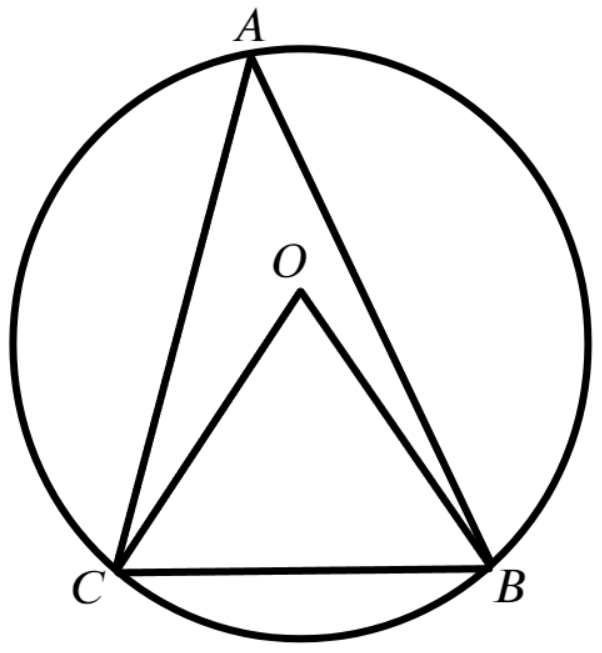
\includegraphics[scale=0.35]{g8-204.png}}
\end{figure}\\
Найдём $\angle A=180^\circ-81^\circ-69^\circ=30^\circ.$ Тогда дуга $BC$ равна $2\cdot30=60^\circ,$ а центральный угол $BOC$ также равен $60^\circ.$ В треугольнике $BOC$ стороны $BO$ и $OC$ равны радиусу, значит он равнобедренный. Так как угол при его вершине равен $60^\circ,$ он равносторонний и $BC=R=5.$\\
